\documentclass[conference,letterpaper]{IEEEtran}
\usepackage{amsmath,amssymb,graphicx,booktabs,url,tikz}
\usetikzlibrary{arrows.meta,positioning}
\begin{document}
\title{Timestamp-Aware Temporal Matching on TUM Revisit Streams:\\A Frozen Negative-Result Study}
\author{\IEEEauthorblockN{Mingyang Zhou}\IEEEauthorblockA{University of Chinese Academy of Sciences\\Empirical working draft; author list subject to confirmation}}
\maketitle
\begin{abstract}
Temporal place recognition can smooth errors while shifting the selected reference away from the current camera location. We study this tradeoff using frozen CosPlace and EigenPlaces descriptors on two continuous TUM RGB-D sequences, with camera-pose labels restricted to offline evaluation. A fixed first-half gallery, a ten-second query buffer, and nearest timestamp association define a reproducible 5Hz revisit protocol. We predeclare 139 mature/simple baseline configurations and 36 timestamp-alignment/endpoint-support configurations on Pioneer SLAM, then freeze settings before one independent Long Office evaluation. The selected constrained refinement matches the strongest development primary count (24/229 at 0.5m), but loses at 0.25m (4/172 versus an envelope of 5/172). On the independent sequence it obtains 34/48 at 0.5m, below the frozen baseline envelope of 35/48, and 0/20 at 0.25m while single-frame EigenPlaces obtains 11/20. It also does not improve the selected time-alignment baseline. These results support a negative finding about this particular refinement mechanism, not a positive method contribution. Small correlated closed-set subsets and substantial open-set coverage gaps limit generalization.
\end{abstract}
\begin{IEEEkeywords}visual place recognition, causal temporal matching, timestamp sampling, reproducibility, negative results\end{IEEEkeywords}
\section{Introduction}
Visual place recognition retrieves earlier images that depict the current location; it supplies candidates for geometric localization rather than a complete six-degree-of-freedom camera pose~\cite{tutorial}. Temporal consistency can reject isolated appearance errors, but aggregate sequence evidence need not place its highest score at the most accurate current endpoint. This distinction matters when a coarse retrieval hit is evaluated using camera-position distances rather than broad frame tolerances.

Previous project iterations used already explored outdoor and ordinal datasets. They remain archived, but cannot constitute independent validation of a newly chosen mechanism. Here we obtain two real continuous RGB streams with publicly documented reference poses~\cite{tum}. Pioneer is the sole development collection; Long Office is not used for algorithm or parameter selection. Our question is narrow: does physical-time score alignment followed by constrained visual endpoint refinement outperform strong short-window and naive local strategies under one fixed metric protocol?

The answer for this bounded study is negative. A small improvement over an old long-window control is insufficient when stronger single-frame, short-window, fusion or simple-refinement comparators exist. Moreover, a gain at 0.5m does not offset a collapse at the predeclared 0.25m sensitivity. We therefore present a reproducible evaluation and failure analysis, not a new state-of-the-art localization algorithm. Our concrete outputs are a timestamp/pose manifest with explicit invalid/open cases, a finite and auditable comparison, one frozen independent test, and image-based inference measurements. Whether this limited empirical contribution is appropriate for a conference requires human scientific review.

\section{Prior Work and Scope}
SeqSLAM and OpenSeqSLAM2 establish sequence trajectory and speed-hypothesis matching~\cite{seqslam,openseq}. STA-VPR uses spatial feature alignment and local-matching dynamic time warping, including relaxed endpoints~\cite{sta}. AdaptSeqVPR describes dynamic sequence-step adjustment and a learned discriminator~\cite{adapt}; our access to that work was limited to publisher abstract/metadata, so we do not claim a full implementation or formula-level distinction. SMR predicts when sequence matching is receptive using supervised score features~\cite{smr}. Temporal alignment, speed handling and endpoint relaxation are therefore established ideas.

We use global CosPlace/EigenPlaces descriptors~\cite{cosplace,eigenplaces}; low-resolution full-image inference is our declared protocol adaptation, not a reproduction of their original published dataset scores. Cosine-score temporal aggregation is likewise not an official reproduction of grayscale SeqSLAM, local-strip STA-VPR, AdaptSeqVPR or the supervised SMR predictor. Our baselines include one-based reciprocal rank fusion with constant 60~\cite{rrf}, fixed affine descriptor-score fusion, and explicit simple local controls. We neither retrain visual models nor introduce a ground-truth-guided online module.

\section{Data and Evaluation Protocol}
\subsection{Acquisition and timestamp association}
Official TUM archives were transferred to Ubuntu after proxy/direct downloads failed; both original network failures and the transferred archive SHA256 values are retained. Full gzip/tar readability, safe paths, mandatory lists, image decoding, pose finiteness and timestamp order were checked before retrieval. Pioneer contains 2,921 RGB images and 44,212 pose rows; Long Office contains 2,585 RGB images and 8,710 pose rows. RGB spans are 155.217s and 87.140s, respectively. The raw depth streams are retained but not used.

TUM reference translations describe the RGB camera optical center in the motion-capture world frame; timestamps are Unix seconds~\cite{tumformat}. Each RGB timestamp is associated with its nearest reference pose within 0.03s; ties choose the earlier pose. Pioneer has ten exact duplicate pose timestamps: we retain all raw rows and differences, and use the first original row for each duplicated time. This deterministic many-to-one association is our evaluation policy, not the official greedy one-to-one association utility. Original timestamps, association deltas, positions, unit quaternions, file hashes and roles are recorded. All 2,921/2,585 PNGs decode; 38/2 RGB rows lack a pose within tolerance. Invalid rows are retained rather than assigned fabricated coordinates.

\subsection{Causal revisit construction}
We retain the earliest RGB image in each floor-based bin relative to the sequence's first acquisition time. The primary rate is 5Hz; 1Hz and 3Hz are predeclared artificial development conditions, not independent recordings. The midpoint of the full raw RGB time span separates the fixed gallery from the query period. Valid-pose sampled images before that midpoint form the gallery; queries start at least ten seconds after it. This creates gallery/query counts 377/339 for Pioneer and 217/168 for Long Office; measured minimum time gaps exceed ten seconds. The initial rule passed the predeclared development minimum of 100 closed queries at 0.5m without adjustment. The rule was accepted before any retrieval, and applied identically to the independent sequence.

Positives are all gallery camera centers within Euclidean 3D distance $r$ of the associated query camera center. We fix $r=0.5$m and sensitivity radii 0.25/1.0m. Orientation does not filter positives. Recall is
\begin{equation}
R@K={1\over N_r}\sum_{i\in C_r}\mathbf{1}[\operatorname{TopK}(i)\cap P_i(r)\ne\varnothing],
\end{equation}
where $C_r$ contains valid-pose queries with at least one positive. Every method shares $C_r$ at each radius, including startup fallback; radii have different denominators, so their percentages are not interchangeable. Pioneer has 338 valid-pose queries and one invalid-pose query. Its closed counts are 172/229/278; open counts are 166/109/60. Long Office has 168 valid queries; closed counts are 20/48/89 and open counts 148/120/79. Invalid-query images still update causal history. We attempt every query and reject none: open queries are forced matches, not successful open-set recognition. No calibrated rejection or full-coverage localization claim is made.

\section{Frozen Matching Strategies}
\subsection{Input, descriptors and index controls}
At query time the input is RGB plus a monotonically increasing acquisition timestamp. A frozen network normalizes and warps the image to 224$\times$224 and produces an L2-normalized 512-D descriptor. Cosine similarity against every earlier gallery descriptor gives current scores $S(t,j)$. Online code cannot receive camera centers, quaternions, ground-truth identities, physical speed or future query scores. Reference timestamps and indices are known prior-map metadata.

The index control uses only current/past observations:
\begin{equation}
T_L(i,j)=\max_{v\in V}{1\over L}\sum_{\ell=0}^{L-1}S(i-\ell,j-\operatorname{rint}(v\ell)),
\end{equation}
with $L\in\{3,5,9\}$ and $V=\{0.8,1,1.2\}$. Out-of-gallery paths are invalid; startup ranks current $S$. The historical fixed L9 uses $v=1.2$. Ties-to-even rounding means L3's three positive ratios can yield identical integer offsets; we do not interpret those as three different effective trajectories. Global blends and local R1/R2 controls use declared fixed weights and identical candidate pools.

\subsection{Timestamp alignment and endpoint constraint}
The timestamp baseline uses five uniformly spaced lags $\delta\in[0,W]$, for $W\in\{0.4,0.8,1.6\}$ seconds. It bilinearly interpolates the score surface using observed current/past query times and known gallery times $\tau_j$:
\begin{equation}
T_W(t,j)=\max_{v\in V_t}{1\over5}\sum_{\delta}\widetilde S(t-\delta,\tau_j-v\delta).
\end{equation}
Here $V_t=\{-1.2,-1,-0.8,0,0.8,1,1.2\}$ contains clock-time ratios, not physical motion estimates. Reverse/stationary hypotheses are given to all timestamp controls as well as the candidate. No extrapolation or future query is used. Query history retains the bracket before the oldest needed lag. Startup uses current $S$ until the physical-time span is available. An independent scalar implementation agrees with the vectorized interpolation on irregular synthetic clocks.

The top $H\in\{1,3\}$ temporal endpoints supply a union of gallery timestamp neighborhoods with half-width $b\in\{0.2,0.4\}$s. Only finite temporal scores enter this common pool $C$. The candidate retains
\begin{equation}
E=\{j\in C:T_W(t,j)\ge\max_kT_W(t,k)-\epsilon\},
\end{equation}
for $\epsilon\in\{0.01,0.03,0.06\}$, ranks $E$ by current $S$, then appends every remaining reference in stable current-score order. Empty/startup cases fall back to $S$. Simple R1 removes the constraint in the same pool; R2 blends current and temporal scores with fixed weights. These controls separate alignment from endpoint refinement. All outputs are complete gallery permutations; the ledgers preserve their top ten IDs and candidate/eligible sets. The score threshold is not a probability or confidence certification.

\subsection{Bounded selection and independent freeze}
We predeclare 139 baseline settings and 36 candidate settings, execute each at developer rates 1/3/5Hz, and introduce no additional branch. Selection maximizes the sum of developer correct@1 at 0.25/0.5m, then primary correct@1, then lexicographic name. The selected candidate is $W=1.6$s, $H=1$, $b=0.2$s, $\epsilon=0.01$; fixed fusion assigns EigenPlaces weight 0.75. A positive claim requires exceeding the baseline envelope at both strict radii in development and independent test. The envelope is a descriptive maximum over frozen comparators, not a test-tuned deployable strategy. Code, loaded-state/checkpoint identities, image manifests, raw-archive hashes, clocks, association, radii, gallery/query rules, methods and timing settings were published in an immutable freeze before the first independent retrieval. A single run evaluates all 139 baselines and the selected candidate. No test-dependent parameter change follows.
\section{Results and Failure Analysis}
\begin{table*}[t]
\centering\caption{Pioneer development (5Hz): radius-specific closed denominators 172, 229, 278. Entries are R@1/5/10 in percent. At 0.5m, 338 valid queries include 109 open queries. Error median/P90 is over all valid queries (metres); time mean/P95 is real batch-one (ms).}
\label{tab:dev}
\scriptsize\setlength{\tabcolsep}{5pt}
\begin{tabular}{lccccc}\hline
Method & 0.25m R1/5/10 & 0.5m R1/5/10 & 1.0m R1/5/10 & Error med/P90 & Time mean/P95\\\hline
CosPlace & 1.7/4.1/5.8 & 10.0/11.4/11.8 & 15.8/16.5/19.1 & 2.25/4.17 & 14.70/15.08 \\
EigenPlaces & 2.3/4.1/6.4 & 10.5/13.1/15.3 & 15.8/19.8/21.9 & 2.20/3.37 & 17.82/18.07 \\
RRF & 2.3/4.1/6.4 & 10.0/11.4/12.7 & 16.2/16.9/17.6 & 2.21/3.69 & 26.35/26.77 \\
Fixed A/B fusion & 2.3/4.1/5.8 & 10.5/12.2/13.5 & 16.5/17.6/19.8 & 2.25/3.56 & 26.38/26.80 \\
Index L3 & 2.9/4.1/5.2 & 9.2/10.9/11.8 & 15.5/16.5/19.1 & 2.25/4.17 & 15.18/15.54 \\
Index L5 & 2.3/3.5/5.2 & 7.4/10.5/10.9 & 14.4/16.5/17.3 & 2.25/4.19 & 15.31/15.63 \\
Index L9 & 2.9/3.5/4.1 & 5.7/6.6/10.0 & 12.9/16.2/16.9 & 2.22/4.09 & 15.55/15.88 \\
Old fixed L9 & 1.2/2.9/3.5 & 5.7/6.6/9.6 & 12.2/13.7/16.2 & 2.22/4.06 & 15.08/15.40 \\
Index global blend & 2.3/4.1/5.2 & 9.6/11.4/11.8 & 15.5/16.9/18.0 & 2.25/4.17 & 15.13/15.39 \\
Index local R1 & 1.7/4.1/6.4 & 10.0/10.9/12.2 & 15.8/16.5/18.0 & 2.25/4.17 & 16.00/16.23 \\
Index local R2 & 2.9/4.1/5.8 & 9.2/10.9/11.8 & 15.8/16.2/19.1 & 2.25/4.18 & 15.98/16.26 \\
Time alignment & 2.3/4.7/5.8 & 10.5/10.9/12.2 & 16.9/20.1/21.2 & 2.25/4.13 & 15.37/15.73 \\
Time local R1 & 2.3/4.1/5.8 & 10.5/10.9/11.8 & 17.3/19.8/22.3 & 2.25/4.13 & 16.11/16.40 \\
Time local R2 & 2.3/4.1/5.8 & 10.5/10.9/11.8 & 17.3/19.8/22.3 & 2.25/4.13 & 16.09/16.37 \\
Constrained refinement & 2.3/4.1/5.8 & 10.5/11.4/11.8 & 16.9/19.8/22.3 & 2.25/4.13 & 16.17/16.56 \\
\hline\end{tabular}\end{table*}
\begin{table*}[t]
\centering\caption{Frozen independent Long Office (5Hz): radius-specific closed denominators 20, 48, 89. Entries are R@1/5/10 in percent. At 0.5m, 168 valid queries include 120 open queries. Error median/P90 is over all valid queries (metres); time mean/P95 is real batch-one (ms).}
\label{tab:test}
\scriptsize\setlength{\tabcolsep}{5pt}
\begin{tabular}{lccccc}\hline
Method & 0.25m R1/5/10 & 0.5m R1/5/10 & 1.0m R1/5/10 & Error med/P90 & Time mean/P95\\\hline
CosPlace & 15.0/60.0/70.0 & 60.4/85.4/100.0 & 82.0/87.6/93.3 & 1.28/4.93 & 14.69/15.04 \\
EigenPlaces & 55.0/90.0/100.0 & 64.6/93.8/97.9 & 88.8/94.4/97.8 & 1.20/4.55 & 17.92/18.21 \\
RRF & 0.0/75.0/95.0 & 64.6/87.5/100.0 & 88.8/92.1/96.6 & 1.22/4.95 & 26.34/26.79 \\
Fixed A/B fusion & 5.0/100.0/100.0 & 66.7/93.8/97.9 & 88.8/93.3/96.6 & 1.22/4.79 & 26.32/26.84 \\
Index L3 & 10.0/55.0/65.0 & 43.8/47.9/72.9 & 80.9/87.6/92.1 & 1.28/4.90 & 15.21/15.57 \\
Index L5 & 0.0/40.0/55.0 & 41.7/45.8/50.0 & 85.4/87.6/92.1 & 1.24/4.88 & 15.26/15.63 \\
Index L9 & 0.0/0.0/0.0 & 27.1/37.5/45.8 & 87.6/88.8/92.1 & 1.22/4.81 & 15.51/15.90 \\
Old fixed L9 & 0.0/0.0/0.0 & 0.0/6.2/39.6 & 80.9/89.9/93.3 & 1.20/4.49 & 15.15/15.45 \\
Index global blend & 5.0/60.0/75.0 & 60.4/77.1/93.8 & 80.9/85.4/91.0 & 1.32/4.94 & 15.24/15.60 \\
Index local R1 & 15.0/60.0/70.0 & 60.4/81.2/93.8 & 82.0/85.4/87.6 & 1.25/4.94 & 15.79/16.14 \\
Index local R2 & 10.0/50.0/70.0 & 47.9/77.1/97.9 & 80.9/86.5/93.3 & 1.29/4.91 & 15.74/16.07 \\
Time alignment & 0.0/60.0/75.0 & 70.8/91.7/100.0 & 85.4/86.5/92.1 & 1.22/4.58 & 15.36/15.79 \\
Time local R1 & 0.0/60.0/70.0 & 68.8/85.4/97.9 & 84.3/88.8/94.4 & 1.22/4.58 & 15.84/16.26 \\
Time local R2 & 0.0/60.0/70.0 & 70.8/85.4/97.9 & 84.3/88.8/94.4 & 1.22/4.58 & 15.83/16.26 \\
Constrained refinement & 0.0/60.0/70.0 & 70.8/85.4/97.9 & 84.3/88.8/94.4 & 1.22/4.58 & 15.90/16.31 \\
\hline\end{tabular}\end{table*}

\subsection{Strong baselines change the apparent conclusion}
At 0.5m the candidate obtains 24/229 developer hits, equal to fixed A/B fusion and several timestamp controls; at 0.25m it obtains 4/172 while the frozen baseline envelope reaches 5/172. The bounded developer gate fails. Long Office gives 34/48 primary hits versus 32/48 for the developer-selected fixed fusion, but the timestamp baseline also gives 34/48 and a simple frozen control gives 35/48. Thus even the primary count does not establish endpoint-refinement benefit over the relevant controls. At 0.25m the candidate gives 0/20, versus 11/20 for single-frame EigenPlaces. We preserve this negative sensitivity rather than change the radius or subset to obtain a favorable method headline.

Each table gives R@1/5/10 at all declared radii. On Long Office the candidate and timestamp baseline tie in primary R@1, but their primary R@5 counts are 41 and 44, respectively. Constrained reranking can harm candidate availability near the top of the list. At 1m their top-one counts are 75 and 76; this wider tolerance cannot repair the failed strict-radii gate. Paired rescue/harm against CosPlace is audited using $N_{\rm rescue}-N_{\rm harm}=N_{\rm correct}-N_{\rm correct,A}$; full query-level differences, candidate coverage and error quantiles are retained, not only selected successes.

\begin{figure}[t]\centering
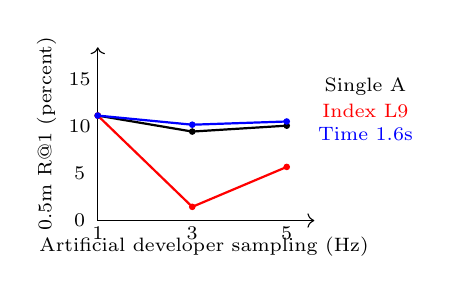
\begin{tikzpicture}[x=1cm,y=1cm]
\draw[->] (0.8,0.35)--(3.55,0.35);\draw[->] (0.8,0.35)--(0.8,2.55);
\node[font=\scriptsize,rotate=90] at (0.15,1.45){0.5m R@1 (percent)};
\node[font=\scriptsize] at (2.15,0.02){Artificial developer sampling (Hz)};
\foreach \x/\label in {0.8/1,2.0/3,3.2/5}{\node[font=\scriptsize] at (\x,0.19){\label};}
\foreach \y/\label in {0.35/0,0.95/5,1.55/10,2.15/15}{\node[font=\scriptsize] at (0.57,\y){\label};}
\draw[black,thick] (0.800,1.683) -- (2.000,1.480) -- (3.200,1.555);
\fill[black] (0.800,1.683) circle (1.2pt);
\fill[black] (2.000,1.480) circle (1.2pt);
\fill[black] (3.200,1.555) circle (1.2pt);
\draw[red,thick] (0.800,1.683) -- (2.000,0.524) -- (3.200,1.031);
\fill[red] (0.800,1.683) circle (1.2pt);
\fill[red] (2.000,0.524) circle (1.2pt);
\fill[red] (3.200,1.031) circle (1.2pt);
\draw[blue,thick] (0.800,1.683) -- (2.000,1.567) -- (3.200,1.608);
\fill[blue] (0.800,1.683) circle (1.2pt);
\fill[blue] (2.000,1.567) circle (1.2pt);
\fill[blue] (3.200,1.608) circle (1.2pt);
\node[font=\scriptsize,text=black] at (4.2,2.05){Single A};
\node[font=\scriptsize,text=red] at (4.2,1.75){Index L9};
\node[font=\scriptsize,text=blue] at (4.2,1.45){Time 1.6s};
\end{tikzpicture}
\caption{Pioneer artificial sampling changes both history duration and gallery coverage. Fixed physical-time alignment is a baseline, not evidence of endpoint-refinement improvement or a new independent collection.}\label{fig:sampling}\end{figure}

\subsection{Sampling, coverage and endpoint interpretation}
Index L9 has developer primary counts 5/45 at 1Hz, 2/138 at 3Hz and 13/229 at 5Hz; the timestamp $W=1.6$s baseline gives 5/45, 14/138 and 24/229. Frame-count windows change their physical duration with sampling, while the time baseline fixes duration. These artificial conditions rebuild both gallery and query and also change spatial reference coverage: they do not isolate timing alone, and they are not independent generalization evidence. The main comparison uses the same 5Hz inputs and common radius-specific query sets.

The primary closed coverage is only 229/338 for Pioneer and 48/168 for Long Office. Forced rankings outside those subsets are visible open-set failures. Position-only positives may depict different viewing directions; frozen global descriptors and a short temporal wrapper cannot be presumed to recover missing visual evidence. Post-test offline orientation diagnosis, without filtering or changing methods, finds that 175/229 Pioneer primary closed queries have no positive reference within 60 degrees of camera rotation; 160 exceed 120 degrees. The median best-positive rotation is 136.95 degrees, compared with 8.70 degrees on Long Office, where 0 primary closed queries exceed 60 degrees. This exposes a position-only protocol difficulty, but does not establish a causal explanation for every retrieval error. We retain the accepted protocol and all difficult queries. Our evaluation measures which earlier camera center was retrieved, not a refined metric camera pose or a geometric correspondence check. Candidate-pool oracle coverage is offline diagnosis only, never an executable method.

\subsection{Actual image inference}
We measured 25,857 complete batch-one query intervals across both streams, 17 frozen representative strategies and three ordered passes per strategy. Each strategy used 20 warm-up images followed by a history reset. The independent CSV aggregation reproduces every mean/P95 and per-pass correct count. Batch-16 cached versus batch-one top-one mismatch count was 0; repeat top-ten mismatches were 0. Batch-size differences are numerical discrepancies to report, not permission to select new methods. Tables show batch-16 cached accuracy and independently measured batch-one latency; the repository includes every actual online pass accuracy. Gallery decoding/encoding and model loading were measured separately. Timing assumes resident models and a cached prior gallery, warm OS file access, and a desktop laptop GPU; it is not a cold-start, embedded-robot or full-SLAM benchmark.

\section{Limitations and Conclusion}
This study uses two short indoor collections with overlapping environments, frozen pretrained global descriptors, a full-image low-resolution warp, and a fixed first-half revisit adaptation of an RGB-D SLAM benchmark. It does not reproduce published descriptor benchmarks, use depth, optimize a visual model or demonstrate robustness across many independent routes. Adjacent frames are correlated; the independent strict subset has only twenty queries. Ratios, support thresholds and model choices were selected on the complete development sequence, so developer performance is exploratory rather than another holdout. Translation-only positives do not guarantee matched orientation. Nearest pose association introduces a finite temporal tolerance; retaining duplicate/invalid evidence is more defensible than silently supplying perfect labels.

We find no support for a positive contribution from the tested constrained endpoint refinement. Physical-time normalization can outperform an old long frame window, yet a stronger simple baseline and strict metric sensitivity defeat a broader improvement claim. Future work requires a separately justified representation/geometry mechanism and a new independent collection if it uses these test results for design. We do not automatically add more weights or repeatedly retune this now-seen test. The present manuscript is an empirical working draft; a method paper is not submission-ready on this evidence alone.

\section*{Reproducibility and AI disclosure}
All V1--V3 originals, earlier negative runs, download failures and manuscript versions are retained. V4 source/configuration, small numeric evidence and checkpoint history are available at \url{https://github.com/zhoumy0313/upinlbs-2026-vpr} on the V4 branch. Original images, weights and large arrays remain local with official sources, SHA256 identities and rebuild instructions. Per-query ledgers independently reproduce counts; table cells are mapped to evidence JSON. Formal authorship, template compliance, copyright, fees and submission remain human decisions.

OpenAI ChatGPT/Codex assisted implementation, command execution, analysis, figures and drafting throughout Sections I--VI. Tool-generated code and prose require author review. Numerical statements here come from retained actual runs; negative results and AI assistance are disclosed. This acknowledgment does not assign authorship to an AI system or imply approval of formal submission.

\begin{thebibliography}{12}
\bibitem{tutorial} S. Schubert, P. Neubert, S. Garg, M. Milford, and T. Fischer, ``Visual place recognition: A tutorial,'' \emph{IEEE Robot. Autom. Mag.}, vol.31, no.3, pp.139--153, 2024.
\bibitem{tum} J. Sturm, N. Engelhard, F. Endres, W. Burgard, and D. Cremers, ``A benchmark for the evaluation of RGB-D SLAM systems,'' in \emph{IROS}, 2012, pp.573--580.
\bibitem{tumformat} TUM Computer Vision Group, ``RGB-D benchmark: File formats and download,'' \url{https://cvg.cit.tum.de/data/datasets/rgbd-dataset/file_formats}, accessed Oct.11,2026.
\bibitem{cosplace} G. Berton, C. Masone, and B. Caputo, ``Rethinking visual geo-localization for large-scale applications,'' in \emph{CVPR}, 2022, pp.4878--4888.
\bibitem{eigenplaces} G. Berton, G. Trivigno, B. Caputo, and C. Masone, ``EigenPlaces: Training viewpoint robust models for visual place recognition,'' in \emph{ICCV}, 2023, pp.11080--11090.
\bibitem{seqslam} M. J. Milford and G. F. Wyeth, ``SeqSLAM: Visual route-based navigation for sunny summer days and stormy winter nights,'' in \emph{ICRA}, 2012, pp.1643--1649.
\bibitem{openseq} B. Talbot, S. Garg, and M. Milford, ``OpenSeqSLAM2.0: An open source toolbox for visual place recognition under changing conditions,'' arXiv:1804.02156, 2018.
\bibitem{sta} F. Lu, B. Chen, X.-D. Zhou, and D. Song, ``STA-VPR: Spatio-temporal alignment for visual place recognition,'' \emph{IEEE Robot. Autom. Lett.}, vol.6, no.3, pp.4297--4304, 2021.
\bibitem{adapt} H. Li, G. Peng, J. Zhang, S. Vaikundam, and D. Wang, ``AdaptSeqVPR: An adaptive sequence-based visual place recognition pipeline,'' in \emph{IROS}, 2023, pp.3284--3289.
\bibitem{smr} S. Hussaini, T. Fischer, and M. Milford, ``Improving visual place recognition with sequence-matching receptiveness prediction,'' in \emph{IROS}, 2025, pp.11073--11080.
\bibitem{rrf} G. V. Cormack, C. L. A. Clarke, and S. B\"uttcher, ``Reciprocal rank fusion outperforms condorcet and individual rank learning methods,'' in \emph{SIGIR}, 2009, pp.758--759.
\end{thebibliography}
\end{document}
